\chapter{Implementierung}
\label{cha:implementation}

% Compiler Architektur Grafik inserten

grammar file -> visitor pattern -> ast ->

Die Implementierung des Compilers ist in zwei Teile aufgeteilt: Frontend und Backend. Die Kommunikation zwischen den beiden Teilen erfolgt mithilfe eines abstrakten Syntaxbaums (AST), welchen das Frontend erzeugt. Dieses Kapitel geht  auf die Architektur und Implementierung dieser Teile ein.

Die Implementierung erfolgt in Kotlin, was das Einbinden von bereits existierende Bibliotheken des JVM Ökosystems problemlos ermöglicht. Konkret geht es dabei um ANTLR und ObjectWeb ASM, welche wichtige Rollen im Compiler übernehmen. Die Möglichkeit, Summentypen in Form von \textit{sealed} Schnittstellen und Klassen implementieren zu können, ermöglicht auch die Abarbeitung des ASTs ungemein.

\begin{figure}[h]
    \caption{Compiler-Architektur}
    \centering
    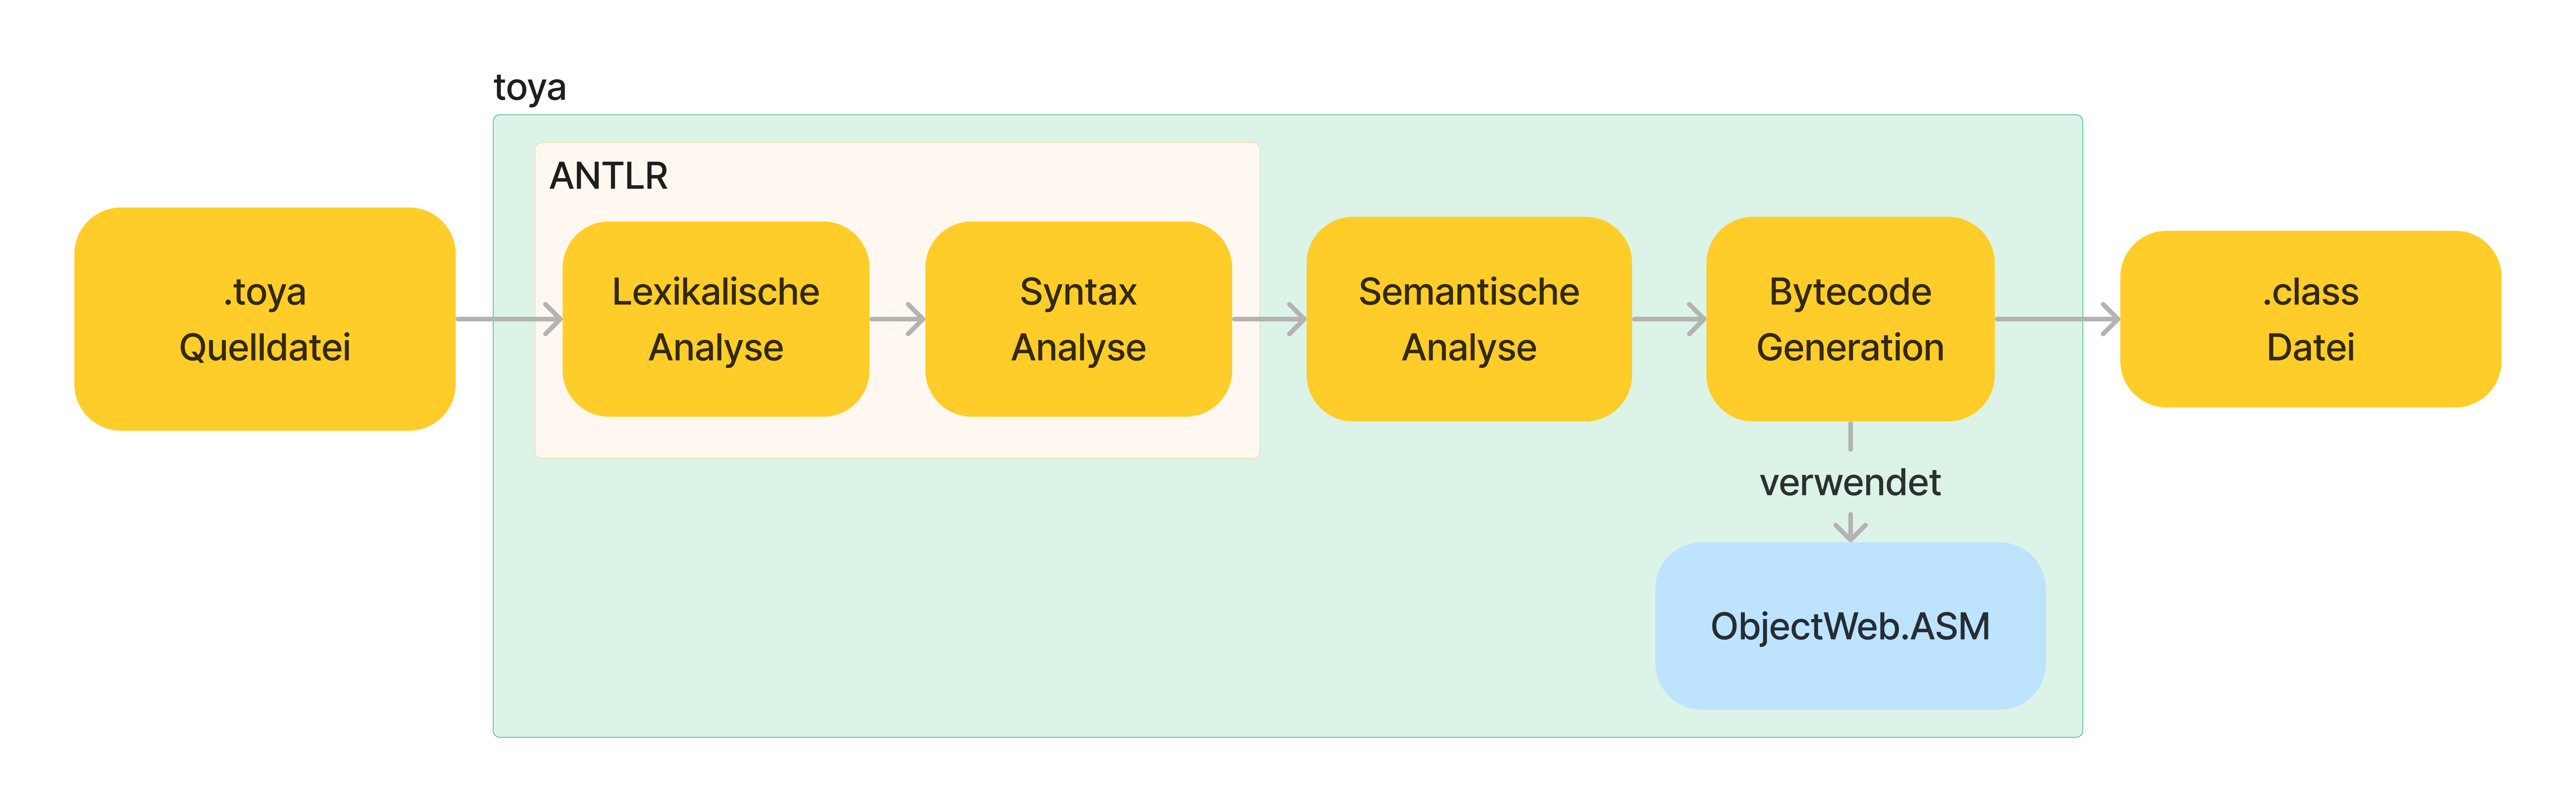
\includegraphics[width=\textwidth]{Compiler.Architecture}
    \label{fig:ibm360}
\end{figure}

\section{Frontend}

Im Frontend erfolgt die lexikalische, syntaktische und teilweise die semantische Analyse. Die lexikalische Analyse zerlegt anhand der bereitgestellten Grammatik den Quellcode in \textit{Token}.

\subsection{Grammatik}

Als Ausgangspunkt des Frontends dient die Grammatik, anhand welcher ANTLR die lexikalische und syntaktische Analyse implementiert. Diese Grammatik definiert die Compiler-Bauer:in in einer \texttt{g4}-Datei. Leerzeichen haben keine semantische Relevanz, weshalb \toya diese in der syntaktischen Analyse überspringt. Als \textit{Token} definiert \toya folgende Zeichen:

\begin{itemize}
    \item Die Schlüsselwörter \texttt{match}, \texttt{for}, \texttt{for}, \texttt{if}, \texttt{else}, \texttt{var}, \texttt{true}, \texttt{false} und \texttt{null}
    \item Die Infix-Operatoren \texttt{>}, \texttt{>=}, \texttt{<}, \texttt{<=}, \texttt{==}, \texttt{!=}, \texttt{\&\&}, \texttt{||} und der Präfix-Operator \texttt{!}
    \item Die arithmetischen Operatoren \texttt{+}, \texttt{-}, \texttt{*} und \texttt{/}
\end{itemize}

Beim Versuch, diese Schlüsselwörter als Variablenname zu Verwenden tritt ein Ausnahmezustand \texttt{VariableNameIsKeywordException} ein. 

\begin{ToyaCode}[numbers=none, caption={Befehl zur Erzeugung der Visitor-Klassen für \toya}]
    antlr4 -o C:\home\Lukas\projects\toya\src\main\java\gen \
    -package gen \
    -Dlanguage=Java \
    -visitor \
    -no-listener \
    -lib C:/home/Lukas/projects/toya/src/main/resources \
    C:/home/Lukas/projects/toya/src/main/resources/toya.g4
\end{ToyaCode}

\subsection{Typ-System}

\subsection{Scope}

Die \texttt{Scope} Klasse ist eine zentrale Komponente in der Verwaltung des AST und wird unter anderem in der semantischen Analyse benötigt. 

\subsection{Abarbeitung des Syntaxbaum}

\subsection{Abstrakter Syntaxbaum}

Die explizite Umwandlung auf einen abstrakten Syntaxbaum ist per se nicht immer nötig, aber da bei \toya ANTLR zum Einsatz kommt und der daraus resultierende Syntaxbaum teilweise zu viel Informationen und teilweise auch Informationen, die nötig wären, nicht enthält, macht es Sinn, diesen Syntaxbaum auf einen abstrakten Syntaxbaum umzubauen.

\section{Backend}

Das Backend erzeugt anhand des AST mithilfe ObjectWeb ASM die \texttt{class}-Datei und Bytecode Anweisungen. Außerdem erfolgt hier der restliche Teil der semantischen Analyse bei welchen Informationen des AST benötigt werden.


% Summen Typen -> sealed class
% Extension Functions und Exapmles wo verwendet
% standard function
% CompositeVisitor
% auf Type System
% AST Struktur
% Defined Compiler Error
% BranchVisitor
% 1 beispielhafter Visitor
% BytecodeGenerator: Compute_FRAMES + COMPUTE_MAXS + classWriter.visit call